\documentclass{article}
\usepackage{graphicx}
\usepackage[utf8]{inputenc}
\usepackage{latexsym,amsfonts,amssymb,amsthm,amsmath}
\usepackage[a4paper,margin=1in]{geometry} % Adjust margins as needed
\usepackage{float}
\usepackage{hyperref}
\usepackage{caption}


\setlength{\parindent}{0in}
\setlength{\oddsidemargin}{0in}
\setlength{\textwidth}{6.5in}
\setlength{\textheight}{8.8in}
\setlength{\topmargin}{0in}
\setlength{\headheight}{18pt}




\begin{document}

	\begin{titlepage}
    	\vspace*{\fill} % Add space before the title block
    	\begin{center}
        	{\huge \textbf{CMU Fall24 16820 Homework 4} \par}
       		\vspace{0.5cm}
        		{\large Patrick Chen \par}
        		\vspace{0.5cm}
		%{\large Collaborators: NA \par}
		%\vspace{0.5cm}
        		{\large October 27, 2024 \par}
    	\end{center}
    	\vspace*{\fill} % Add space after the title block to center everything
	\end{titlepage}
	
	\newpage
	\subsection*{Q1.1 at page 3}
	Ans:\\
	\hangindent=1.5em \hspace{1.5em} We have the following equation:\\
	\begin{align}
		\text{softmax}(\mathbf{x} + c)  &= \frac{e^{x_i+c}}{\sum_j e^{x_j+c}} \\
		&= \frac{e^ce^{x_i}}{e^c\sum_j e^{x_j}} \\
		&= \frac{e^{x_i}}{\sum_j e^{x_j}}\\
		&= \text{softmax}(\mathbf{x})
	\end{align}
	The idea to use c = -$max_{x_i}$ is beneficial because we can have more numerical stablility as the value of $e^{x_i-max_{x_{i}}}$ in softmax would be in the range from 0 to 1, avoiding the risk of overflow.

	\newpage
	\subsection*{Q1.2 at page 3}
	Ans:\\
	\hangindent=1.5em \hspace{1.5em} The range of each element, $\frac{e^{x_i}}{\sum e^{x_i}}$ is from 0 to 1, the sum over all elements would be 1, because  $\sum \frac{e^{x_i}}{\sum e^{x_i}} = \frac{\sum e^{x_i}}{\sum e^{x_i}} = 1$. \newline
	\newline
	\hangindent=1.5em \hspace{1.5em} One could say that “\textit{softmax takes an arbitrary real-valued vector $\mathbf{x}$ and turns it into a} \underline{probability distribution}”. \newline
	\newline
	\hangindent=1.5em \hspace{1.5em} The first step: $s_i = e^{x_i}$ transforms $x_i$ to a positive value, representing the frequency of $x_i$. The second step: $S = \sum s_i$ can be deemed as a normalization to ensure the sum of output probability equals to 1, and it can also be deemed as the total frequency of each dimension $x_i$ in $\mathbf{x}$. The third step: $softmax(x_i) = \frac{1}{S}S_i$ calculates the ratio of frequency of each element $x_i$ among all the dimensions in $\mathbf{x}$, indicating the probability, where each element is between 0 and 1, and the summation across all of each element is 1.

	\newpage
	\subsection*{Q1.3 at page 3}
	Ans:\\
	\hangindent=1.5em \hspace{1.5em} When using multi-layer neural networks without a non-linear activation function, we would have (Assuming n layers fully connected neural network):
	\begin{align}
		y &= W_nx_n + b_n \\
		&= W_n(W_{n-1}x_{n-1} + b_{n-1}) + b_n\\
		&= W_nW_{n-1}x_{n-1} + W_nb_{n-1} + b_n\\
		&= W_nW_{n-1}(W_{n-2}(......(W_1x_{1} + b_1))) + W_nb_{n-1} + b_n \\
		&= W^{'}x^{'} + b^{'}, where \hspace{1mm} W^{'} = W_{n}W_{n-1}...W_1, \hspace{1mm}x^{'} = x_{1}, \hspace{1mm}b^{'} = W_nW_{n-1}...W_{2}b_1 + ... + W_{n}b_{n-1} + b_n
	\end{align}	
	As we can see in equation (9) above, it is still a linear regression.
	
	\newpage
	\subsection*{Q1.4 at page 3}
	Ans:\\
	\hangindent=1.5em \hspace{1.5em}
	\begin{align}
		\frac{d \sigma(x)}{dx} &= \frac{d}{dx} \frac{1}{1 + e^{-x}} \\
		&= \frac{e^{-x}}{(1+e^{-x})^2} \\
		&= \frac{e^{-x}}{(1+e^{-x})(1+e^{-x})} \\
		&= \frac{e^{-x}}{(1+e^{-x})} \frac{1}{(1+e^{-x})}\\
		&= (1-\sigma(x))\sigma(x)
	\end{align}		
	
	\newpage
	\subsection*{Q1.5 at page 3}
	Ans:\\
	\hangindent=1.5em \hspace{1.5em}
	\begin{align}
		\frac{\partial J}{\partial W} &= \frac{\partial J}{\partial y} \frac{\partial y}{\partial W}\\
		&= \delta \hspace{1mm} x^T \in \mathbb{R}^{k \times d} \\
		\frac{\partial J}{\partial x} &= \frac{\partial J}{\partial y} \frac{\partial y}{\partial x}\\
		&= W^T \delta \in \mathbb{R}^{d \times 1}\\
		\frac{\partial J}{\partial b} &= \frac{\partial J}{\partial y} \frac{\partial y}{\partial b}\\
		&= \delta \circ \mathbf{1}_k, \text{where $\circ$ is the element-wised multiplication, and $\mathbf{1}_k$ is a kx1 vector with all elements set to 1.} \\
		&= \delta \in \mathbb{R}^{k \times 1}
	\end{align}
	
	\newpage
	\subsection*{Q1.6 at page 3}
	Ans:\\
	\hangindent=1.5em \hspace{1.5em}
	\begin{enumerate}
		\item As we can see from the below plot of the derivative of sigmoid function, the value of $(1-\sigma(x))\sigma(x)$ is in range [0, 0.25]. If we have multiple layers neural network applying sigmoid activation function, then during the backpropagation, we would need to multiply $(1-\sigma(x))\sigma(x)$ many times from the output layer to the input layer to get the gradient of weight, and the maximum of the value would be $0.25^n$, assuming we have n hidden layers. This value would be very small, nearly zero, resulting in the vanishing of gradient.\\
		
		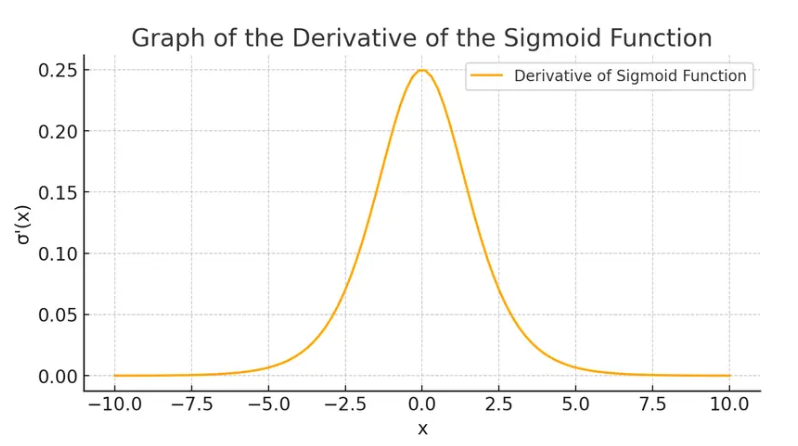
\includegraphics[width=0.5\textwidth]{./Q1_6_plot1.png}
		
		\item The output range of tanh(x) is [-1, 1], and the output range of sigmoid function is [0, 1]. We prefer tanh because it has wider range around zero, and it can map input x to either positive or negative values, reducing the bias introduced by sigmoid only outputting positive activation values.
		\item As we can see from the below figure, the $tanh^{'}(x)$ has value nearly 1 for inputs near zero, which is much more larger than the value of 0.25 of $\sigma^{'}(x)$ (from above figure in problem 1) when inputs near zero. This means that tanh(x) has less of a vanishing gradient problem.
		
		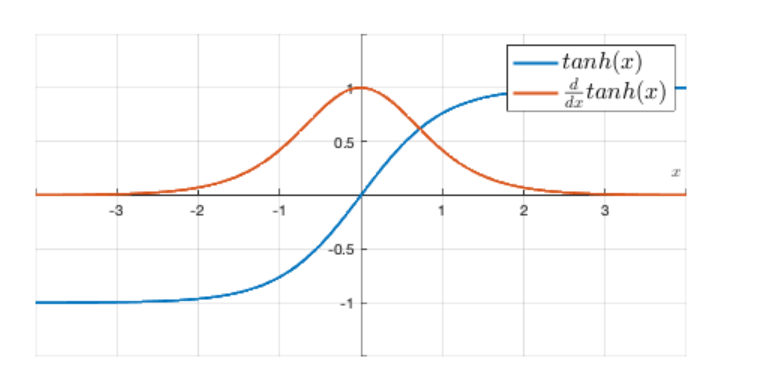
\includegraphics[width=0.5\textwidth]{./Q1_6_plot2.png}
	
		\item The derivation of tanh(x) in terms of $\sigma$(x) is shown below:
		\begin{align}
			tanh(x) &= \frac{1-e^{-2x}}{1+e^{-2x}} \\
			&= \frac{1}{1+e^{-2x}} + (-\frac{e^{-2x}}{1+e^{-2x}}) \\
			&= \sigma(2x) - (1-\sigma(2x))\\
			&= 2\sigma(2x)-1
		\end{align}		
		
	\end{enumerate}	
	
	\newpage
	\subsection*{Q2.1.1 at page 4}
	Ans:\\
	\hangindent=1.5em \hspace{1.5em} When weights are initialized to zero, then in forward propagation, all the output of layers would have the same zero value. Then during the back propagation, all the weights would have same gradients, and it means that each neuron in each layer is trying to learn the same feature, failing to capture the variation and complexity in each dimension of data. The result would be the model fails to converge to a effective solution.

	\newpage
	\subsection*{Q2.1.2 at page 4}
	Ans:\\
	\hangindent=1.5em \hspace{1.5em} The following \autoref{fig:Q212_cns} shows the code snippet of initialize\_weights() in the nn.py:
	\newline

	\begin{minipage}{1\linewidth}
		\centering
		\hspace{0.12\linewidth} 
		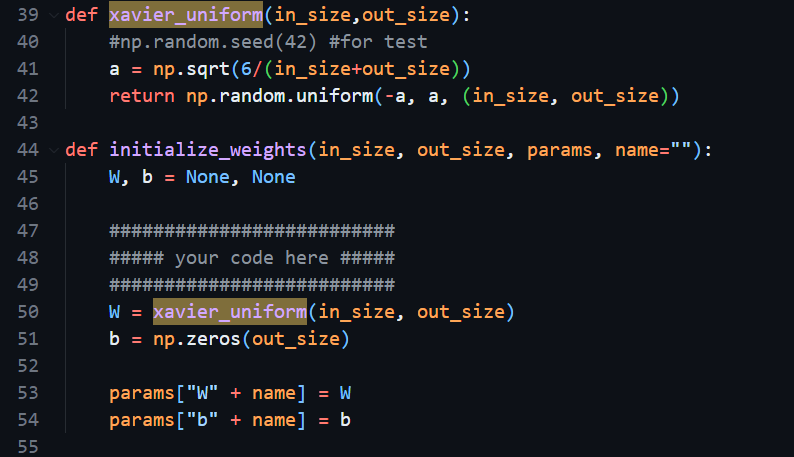
\includegraphics[width=0.7\linewidth]{./Q2_1_2_cns.png}  % Adjust the width to 50% of the line width
		\refstepcounter{figure}  % Increment the figure counter
		\newline
		\textbf{Figure \thefigure:} Code Snippet % Manually add a caption/title
		\label{fig:Q212_cns}  % Label for referencing
	\end{minipage}
	
	\newpage
	\subsection*{Q2.1.3 at page 4}
	Ans:\\
	\hangindent=1.5em \hspace{1.5em} Initializing the weight with random numbers helps the neural network learn different features and pattern in data and facilitate the searching for an optimal point that minimize the loss. Scaling the initialization depending on the layer size could help the output of forward and backward propagation of each layer have the same variance as the input, helping stabilizing the output values and avoid gradient vanishing and explosion.	
	
	\newpage
	\subsection*{Q2.2.1 at page 4}
	Ans:\\
	\hangindent=1.5em \hspace{1.5em}  The following \autoref{fig:Q221_cns} shows the code snippet of sigmoid() and forward() in the nn.py:
	\newline
	
	\begin{minipage}{1\linewidth}
		\centering
		\hspace{0.12\linewidth} 
		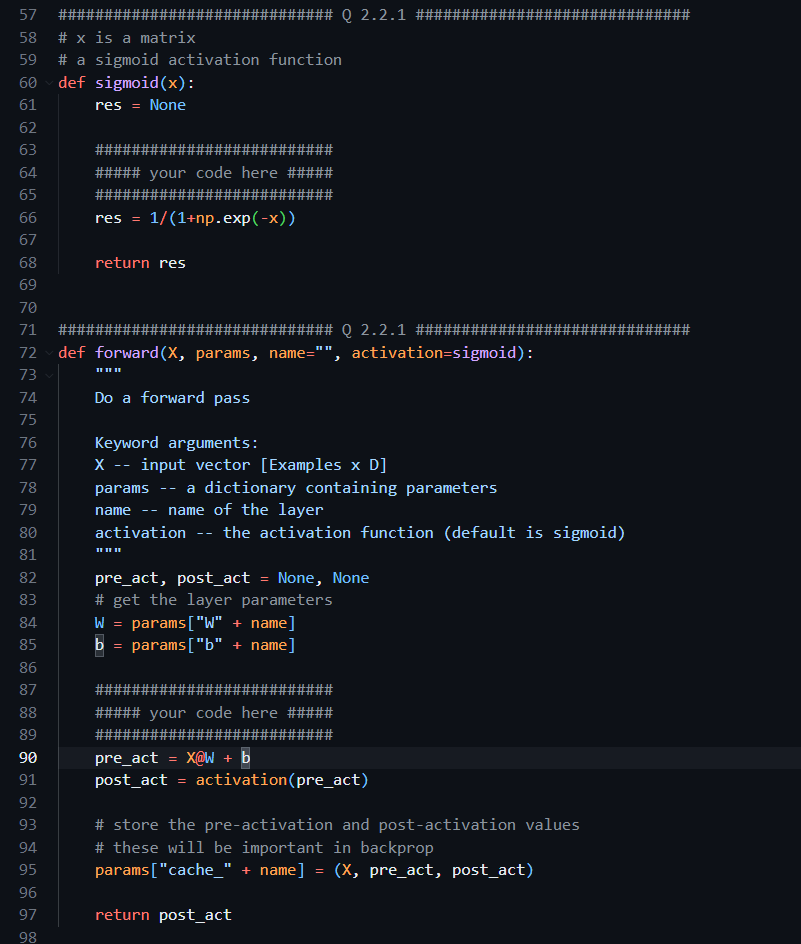
\includegraphics[width=0.7\linewidth]{./Q221_cns.png}  % Adjust the width to 50% of the line width
		\refstepcounter{figure}  % Increment the figure counter
		\newline
		\textbf{Figure \thefigure:} Code Snippet of sigmoid() and forward()% Manually add a caption/title
		\label{fig:Q221_cns}  % Label for referencing
	\end{minipage}	
	
	\newpage
	\subsection*{Q2.2.2 at page 4}
	Ans:\\
	\hangindent=1.5em \hspace{1.5em}  The following \autoref{fig:Q222_cns} shows the code snippet of softmax() in the nn.py:
	\newline

	\begin{minipage}{1\linewidth}
		\centering
		\hspace{0.12\linewidth} 
		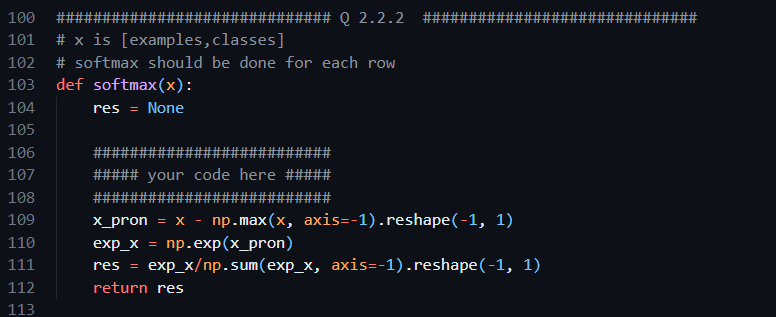
\includegraphics[width=0.7\linewidth]{./Q222_cns.png}  % Adjust the width to 50% of the line width
		\refstepcounter{figure}  % Increment the figure counter
		\newline
		\textbf{Figure \thefigure:} Code Snippet of softmax() % Manually add a caption/title
		\label{fig:Q222_cns}  % Label for referencing
	\end{minipage}	
	
	\newpage
	\subsection*{Q2.2.3 at page 4}
	Ans:\\
	\hangindent=1.5em \hspace{1.5em}  The following \autoref{fig:Q223_cns} shows the code snippet of compute\_loss\_and\_acc() in the nn.py:
	\newline

	\begin{minipage}{1\linewidth}
		\centering
		\hspace{0.12\linewidth} 
		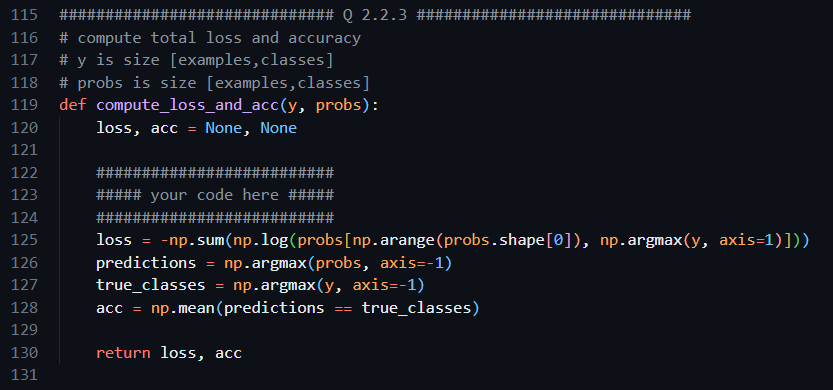
\includegraphics[width=0.7\linewidth]{./Q223_cns.png}  % Adjust the width to 50% of the line width
		\refstepcounter{figure}  % Increment the figure counter
		\newline
		\textbf{Figure \thefigure:} Code Snippet of compute\_loss\_and\_acc() % Manually add a caption/title
		\label{fig:Q223_cns}  % Label for referencing
	\end{minipage}	
	
	\newpage
	
	\subsection*{Q2.3 at page 5}
	Ans:\\
	\hangindent=1.5em \hspace{1.5em}  The following \autoref{fig:Q23_cns} shows the code snippet of backwards() in the nn.py:
	\newline

	\begin{minipage}{1\linewidth}
		\centering
		\hspace{0.12\linewidth} 
		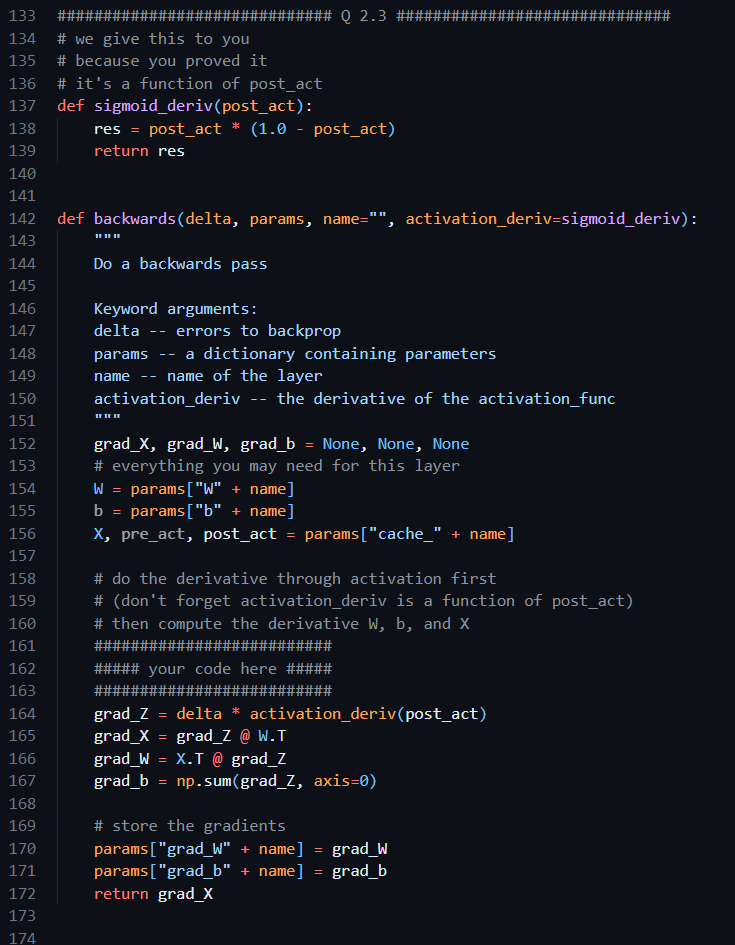
\includegraphics[width=0.7\linewidth]{./Q23_cns.png}  % Adjust the width to 50% of the line width
		\refstepcounter{figure}  % Increment the figure counter
		\newline
		\textbf{Figure \thefigure:} Code Snippet of backwards() % Manually add a caption/title
		\label{fig:Q23_cns}  % Label for referencing
	\end{minipage}	
	\newpage	
	
	\subsection*{Q2.4 at page 5}
	Ans:\\
	\hangindent=1.5em \hspace{1.5em}  The following \autoref{fig:Q24_cns} and \autoref{fig:Q24_cns2} shows the code snippet of get\_random\_batch() in nn.py and training loop procedure in run\_q2.py:
	\newline	
	
	\begin{minipage}{0.48\linewidth}
		\centering
		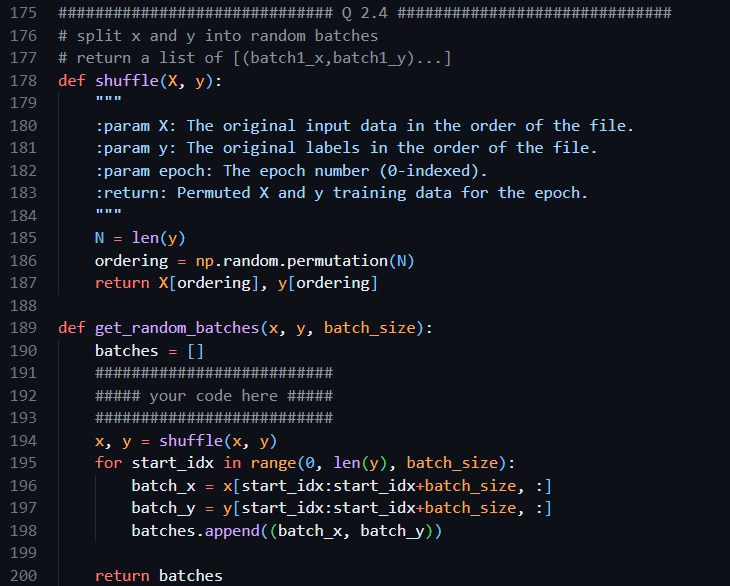
\includegraphics[width=\linewidth]{./Q24_cns.png}
		\refstepcounter{figure}  % Increment the figure counter
		\textbf{Figure \ref{fig:Q24_cns}:} Code Snippet of Random Batch % Manually add a caption/title
		\label{fig:Q24_cns}         % Label for referencing	
	\end{minipage}
	\hfill
	\begin{minipage}{0.48\linewidth}
		\centering
		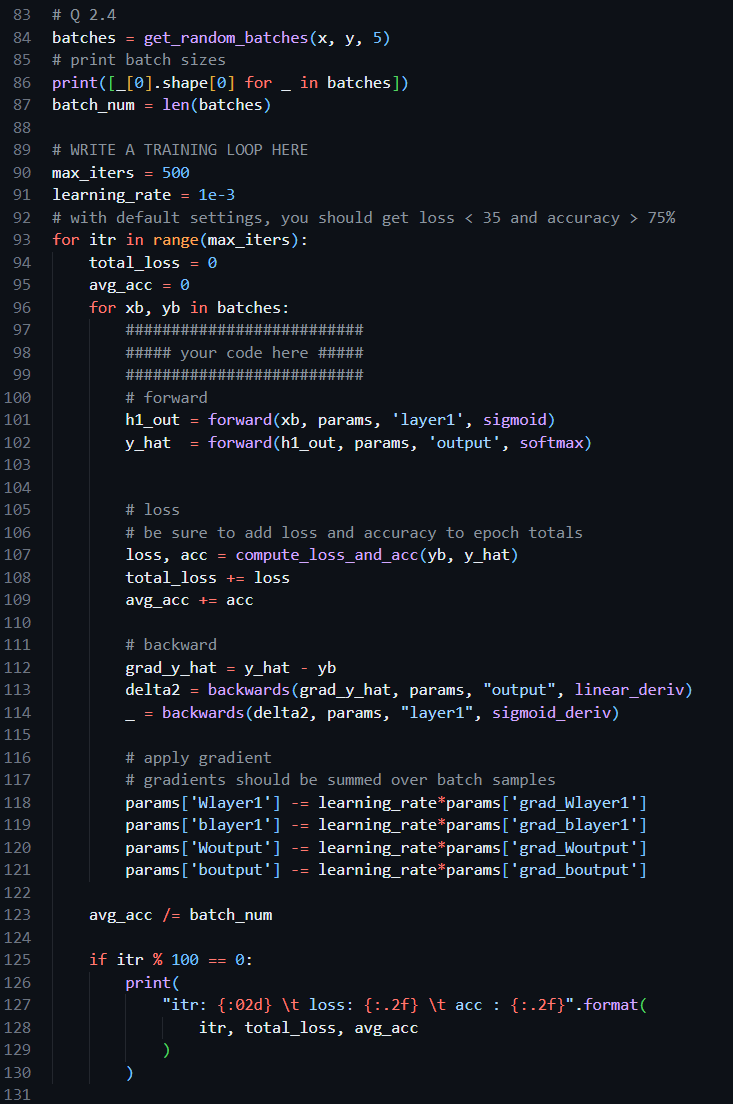
\includegraphics[width=\linewidth]{./Q24_cns2.png}
		\refstepcounter{figure}  % Increment the figure counter
		\textbf{Figure \ref{fig:Q24_cns2}:} Code Snippet of Training Loop  % Manually add a caption/title
		\label{fig:Q24_cns2}         % Label for referencing
	\end{minipage}	
	
	\newpage
	\subsection*{Q2.5 at page 5}
	Ans:\\
	\hangindent=1.5em \hspace{1.5em}  The following \autoref{fig:Q25_cns} shows the code snippet of finite difference in run\_q2.py:
	\newline

	\begin{minipage}{1\linewidth}
		\centering
		\hspace{0.12\linewidth} 
		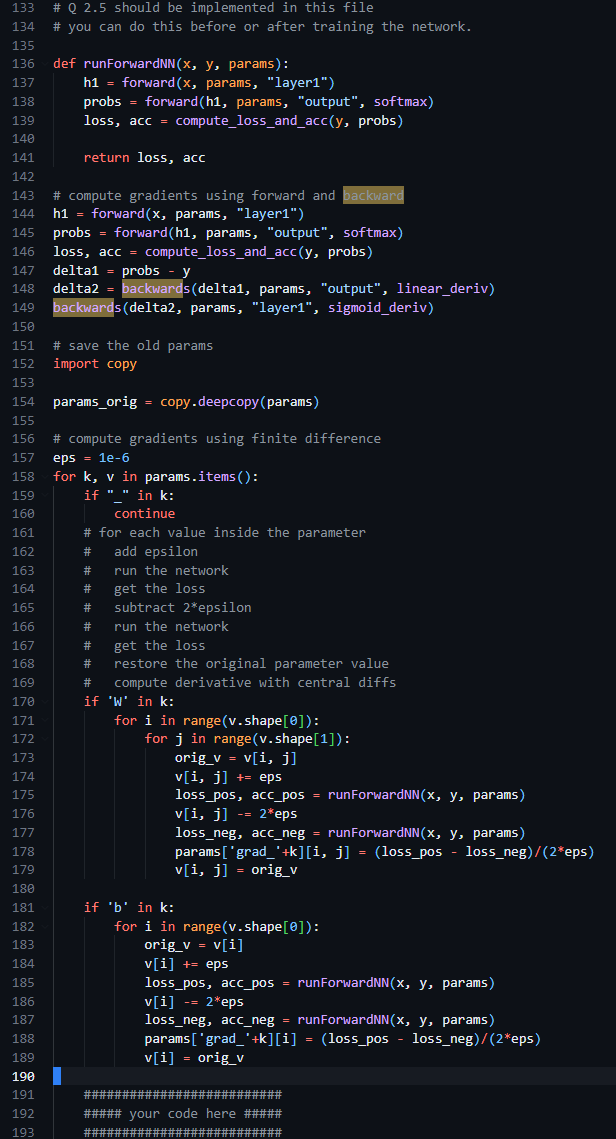
\includegraphics[width=0.7\linewidth, height=1.2\columnwidth]{./Q25_cns.png}  % Adjust the width to 50% of the line width
		\refstepcounter{figure}  % Increment the figure counter
		\newline
		\textbf{Figure \thefigure:} Code Snippet of Finite Difference Gradient Check % Manually add a caption/title
		\label{fig:Q25_cns}  % Label for referencing
	\end{minipage}	
	
	\newpage
	\subsection*{Q3.1 at page 6}
	Ans:\\
	\hangindent=1.5em \hspace{1.5em}  The following \autoref{fig:Q31_res1} and \autoref{fig:Q31_res2} shows the result after 100 epochs training with batch size set to 64, and learning rate set to $2e^{-3}$. The validation accuracy is 77\%.'
	\newline	

	\begin{minipage}{0.48\linewidth}
		\centering
		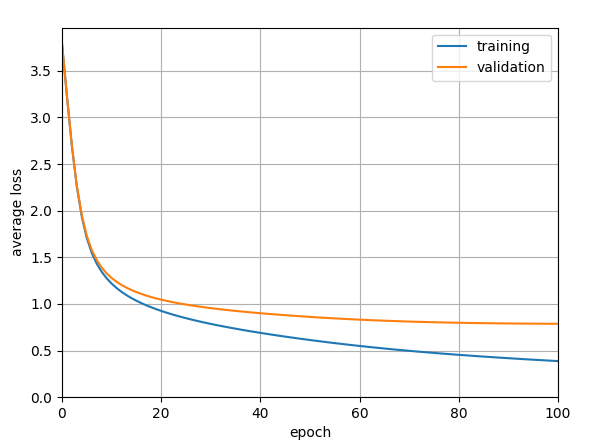
\includegraphics[width=\linewidth]{./Q31_res_loss.png}
		\refstepcounter{figure}  % Increment the figure counter
		\textbf{Figure \ref{fig:Q31_res1}:} Average Loss vs Epoch % Manually add a caption/title
		\label{fig:Q31_res1}         % Label for referencing	
	\end{minipage}
	\hfill
	\begin{minipage}{0.48\linewidth}
		\centering
		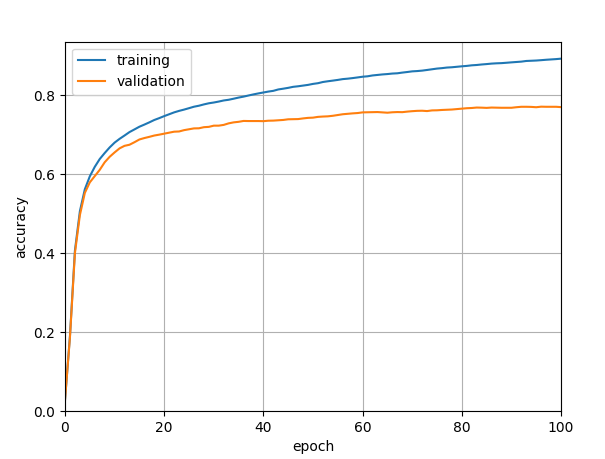
\includegraphics[width=\linewidth]{./Q31_res_acc.png}
		\refstepcounter{figure}  % Increment the figure counter
		\textbf{Figure \ref{fig:Q31_res2}:} Accuracy vs Epoch  % Manually add a caption/title
		\label{fig:Q31_res2}         % Label for referencing
	\end{minipage}		
	
	\newpage
	\subsection*{Q3.2 at page 6}
	Ans:\\
	All of the following results are generated with batch size = 64.\newline
	\hangindent=1.5em \hspace{1.5em} The following \autoref{fig:Q32_lr1_res1} and \autoref{fig:Q32_lr1_res2} shows the result of learning rate set to the ten times of tuned one in Q3.1, which is $2e^{-2}$. The test accuracy is 72.22\%, lower than the case of tuned learning rate in Q3.1. The plots show sawtooth-like pattern, indicating the learning rate is set too high, making the gradient update and the loss change drastic.
	\newline	

	\begin{minipage}{0.48\linewidth}
	\centering
	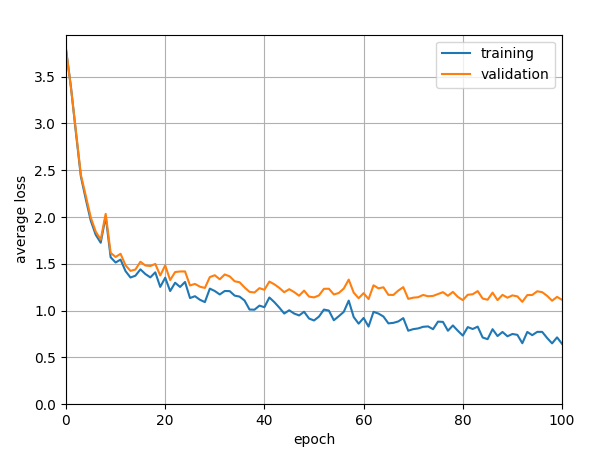
\includegraphics[width=\linewidth]{./Q32_lr1_res1.png}
	\refstepcounter{figure}  % Increment the figure counter
	\textbf{Figure \ref{fig:Q32_lr1_res1}:} Average Loss vs Epoch % Manually add a caption/title
	\label{fig:Q32_lr1_res1}         % Label for referencing	
	\end{minipage}
\hfill
	\begin{minipage}{0.48\linewidth}
	\centering
	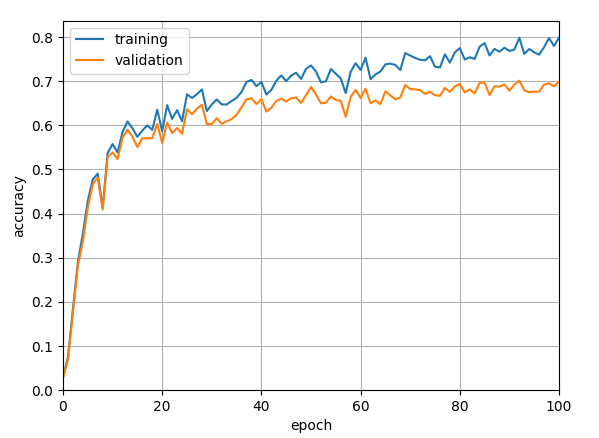
\includegraphics[width=\linewidth]{./Q32_lr1_res2.png}
	\refstepcounter{figure}  % Increment the figure counter
	\textbf{Figure \ref{fig:Q32_lr1_res2}:} Accuracy vs Epoch  % Manually add a caption/title
	\label{fig:Q32_lr1_res2}         % Label for referencing
	\end{minipage}	
	\newline
	\newline
	
	\hangindent=1.5em \hspace{1.5em}The following \autoref{fig:Q32_lr2_res1} and \autoref{fig:Q32_lr2_res2} show the result of the tuned learning rate set to the same as Q3.1, which is $2e^{-3}$. The result is the best, having test accuracy 77.83\%.
	\newline		
	
	\begin{minipage}{0.48\linewidth}
	\centering
	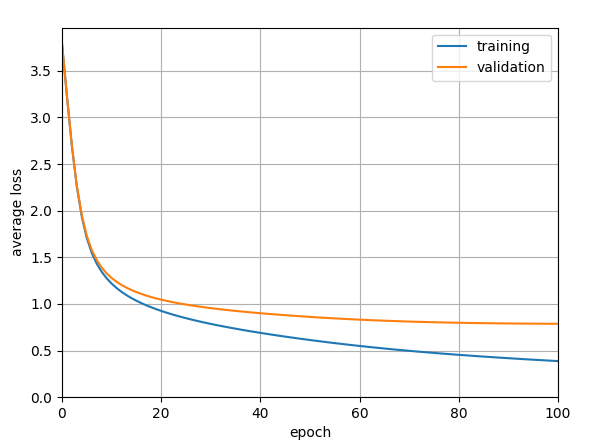
\includegraphics[width=\linewidth]{./Q31_res_loss.png}
	\refstepcounter{figure}  % Increment the figure counter
	\textbf{Figure \ref{fig:Q32_lr2_res1}:} Average Loss vs Epoch % Manually add a caption/title
	\label{fig:Q32_lr2_res1}         % Label for referencing	
	\end{minipage}
\hfill
	\begin{minipage}{0.48\linewidth}
	\centering
	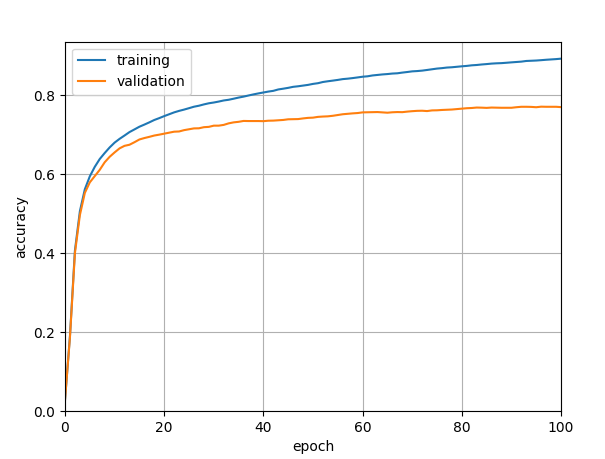
\includegraphics[width=\linewidth]{./Q31_res_acc.png}
	\refstepcounter{figure}  % Increment the figure counter
	\textbf{Figure \ref{fig:Q32_lr2_res2}:} Accuracy vs Epoch  % Manually add a caption/title
	\label{fig:Q32_lr2_res2}         % Label for referencing
	\end{minipage}		
	\newline
	\newline
	
	\hangindent=1.5em \hspace{1.5em}The following \autoref{fig:Q32_lr3_res1} and \autoref{fig:Q32_lr3_res2} show the result of learning rate set to one tenth of the one set in Q3.1, which is $2e^{-4}$. The test accuracy is 69\%, lower than the tuned case in Q3.1. The plots show that the model has not yet reached the convergence point because of the small learning rate. There is still room for improvement, and we need more epochs to optimize this model.
	\newline		
	
	\begin{minipage}{0.48\linewidth}
	\centering
	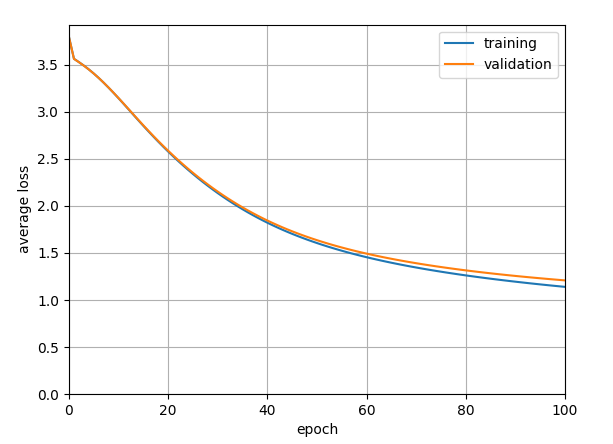
\includegraphics[width=\linewidth]{./Q32_lr3_res1.png}
	\refstepcounter{figure}  % Increment the figure counter
	\textbf{Figure \ref{fig:Q32_lr3_res1}:} Average Loss vs Epoch % Manually add a caption/title
	\label{fig:Q32_lr3_res1}         % Label for referencing	
	\end{minipage}
\hfill
	\begin{minipage}{0.48\linewidth}
	\centering
	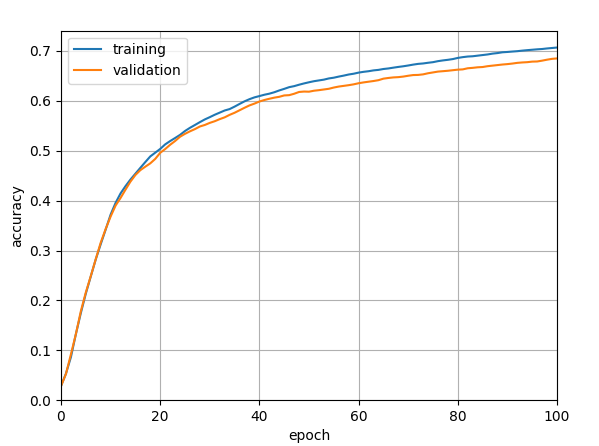
\includegraphics[width=\linewidth]{./Q32_lr3_res2.png}
	\refstepcounter{figure}  % Increment the figure counter
	\textbf{Figure \ref{fig:Q32_lr3_res2}:} Accuracy vs Epoch  % Manually add a caption/title
	\label{fig:Q32_lr3_res2}         % Label for referencing
	\end{minipage}	
	
	\newpage
	\subsection*{Q3.3 at page 6}
	Ans:\\
	\hangindent=1.5em \hspace{1.5em}The following \autoref{fig:Q33_res1} shows the initialized weight that looks like noise, which is expected because we initialized the weighted as random uniform distribution. The \autoref{fig:Q33_res2} shows the optimized weight after 100 epochs, demonstrating more clear patterns.


	\begin{minipage}{0.48\linewidth}
	\centering
	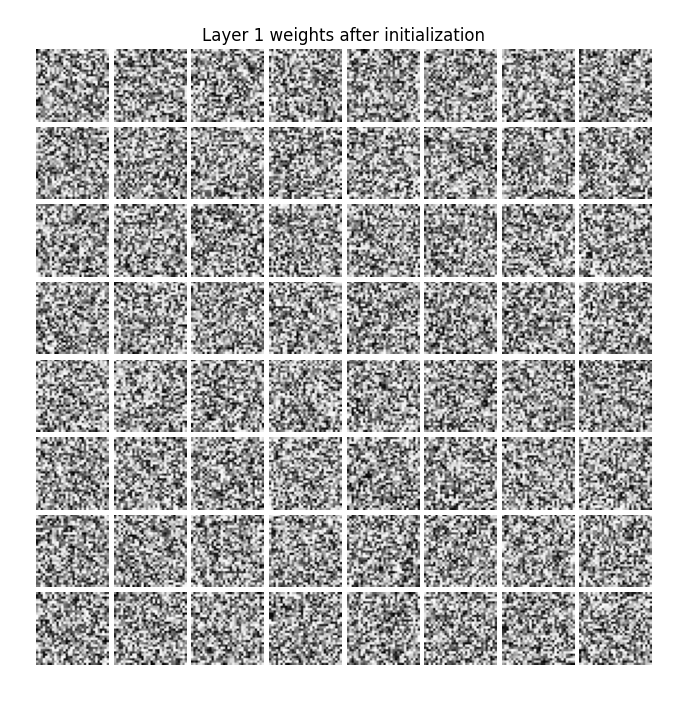
\includegraphics[width=\linewidth]{./Q33_res1.png}
	\refstepcounter{figure}  % Increment the figure counter
	\textbf{Figure \ref{fig:Q33_res1}:} Layer1 Weights Initialization % Manually add a caption/title
	\label{fig:Q33_res1}         % Label for referencing	
	\end{minipage}
	\hfill
	\begin{minipage}{0.48\linewidth}
	\centering
	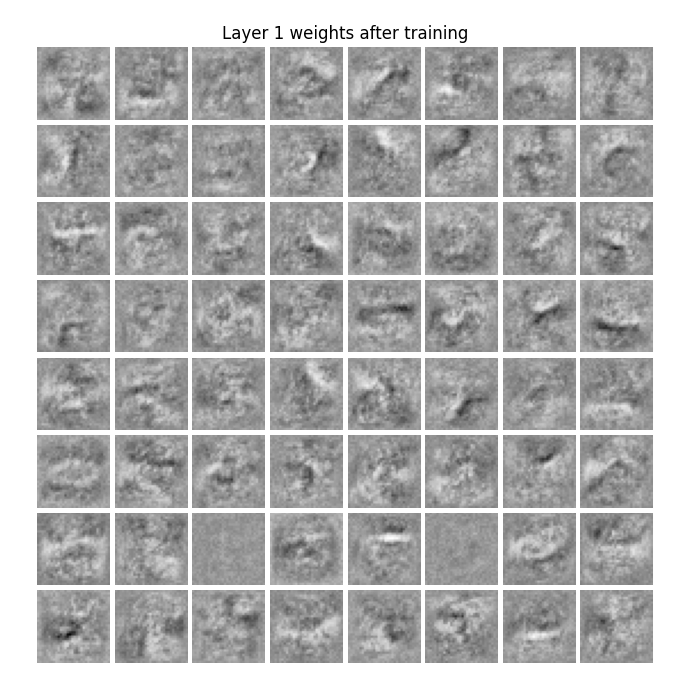
\includegraphics[width=\linewidth]{./Q33_res2.png}
	\refstepcounter{figure}  % Increment the figure counter
	\textbf{Figure \ref{fig:Q33_res2}:} Layer1 Weights After Training  % Manually add a caption/title
	\label{fig:Q33_res2}         % Label for referencing
	\end{minipage}		
	
	\newpage
	\subsection*{Q3.4 at page 6}
	Ans:\\
	\hangindent=1.5em \hspace{1.5em}The	\autoref{fig:Q34_res} shows the confusion matrix of my best model: learning rate = $2e^{-3}$, batch size = 64, epochs = 100. Some top pairs of classes that are most commonly confused are: 'O' and '0', '5' and 'S', '2' and 'Z', 'I' and '1'.
	\newline

\begin{minipage}{1\linewidth}
	\centering
	\hspace{0.12\linewidth} 
	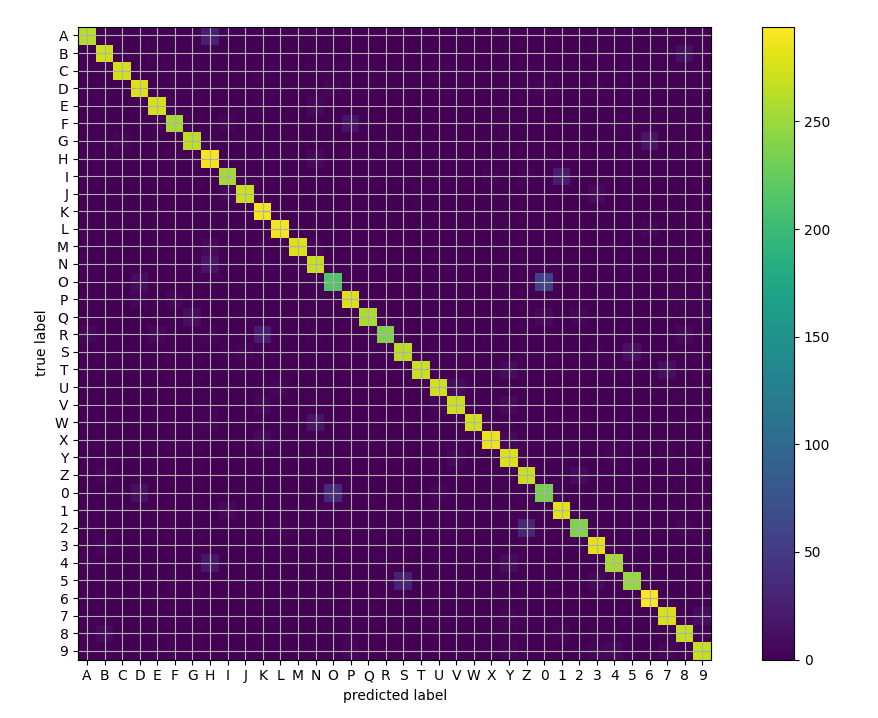
\includegraphics[width=0.7\linewidth]{./Q34_res.png}  % Adjust the width to 50% of the line width
	\refstepcounter{figure}  % Increment the figure counter
	\newline
	\textbf{Figure \thefigure:} Confusion Matrix of Best Model % Manually add a caption/title
	\label{fig:Q34_res}  % Label for referencing
\end{minipage}	

	\newpage
	\subsection*{Q4.1 at page 8\texttt{}}
	Ans:\\
	\hangindent=1.5em \hspace{1.5em}Two assumptions are made as the following:
	\begin{itemize}
		\item Each individual letter is a connected component. In the step2 of the method outlined at page 7 in the hw4.pdf, the connected component is used, indicating that each letter should be a connected component, otherwise, the method would fail. For example, \autoref{fig:Q41_ex1} may fail to extract each individual letter because of not being connected component:
		\newline
		\begin{minipage}{1\linewidth}
			\centering
			\hspace{0.12\linewidth} 
			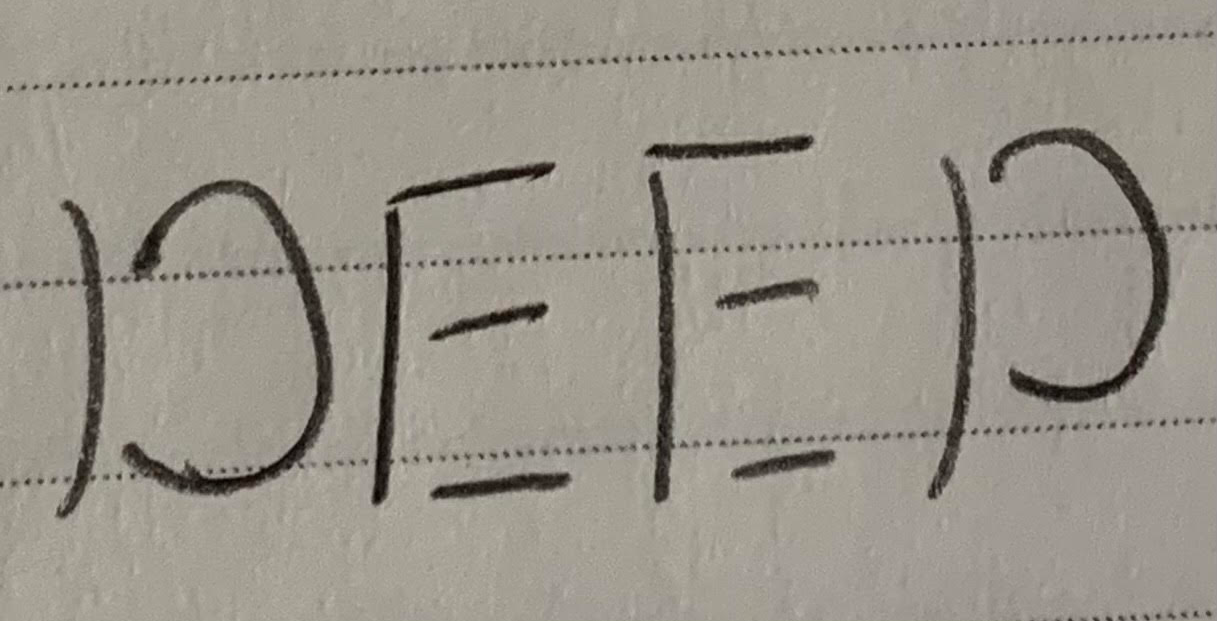
\includegraphics[width=0.4\linewidth]{./Q41_ex1.png}  % Adjust the width to 50% of the line width
			\refstepcounter{figure}  % Increment the figure counter
			\newline
			\textbf{Figure \thefigure:} Example1 of Fail % Manually add a caption/title
			\label{fig:Q41_ex1}  % Label for referencing
		\end{minipage}
		\newline
		
		\item There should not be any connection between two individual letters. As in the step2 to grep the connected component as a letter, two individual letters should not be connected, otherwise, there may be failure on separating them. For example the \autoref{fig:Q41_ex2} may fail to extract each letter due to some connection between individual letters, such as 'A' and 'C', 'C' and 'H', 'E' and 'A', ..., and so on:
		\newline
		
		\begin{minipage}{1\linewidth}
		\centering
		\hspace{0.12\linewidth} 
		
\includegraphics[width=0.7\linewidth]{./Q41_ex2.png}  % Adjust the width to 50% of the line width
		\refstepcounter{figure}  % Increment the figure counter
		\newline
		\textbf{Figure \thefigure:} Example2 of Fail % Manually add a caption/title
		\label{fig:Q41_ex2}  % Label for referencing
		\end{minipage}		
	\end{itemize}
	
	\newpage
	\subsection*{Q4.2 at page 8\texttt{}}
	Ans:\\
	\hangindent=1.5em \hspace{1.5em}  The following \autoref{fig:Q42_cns} shows the code snippet:
	\newline

	\begin{minipage}{1\linewidth}
	\centering
	\hspace{0.12\linewidth} 
	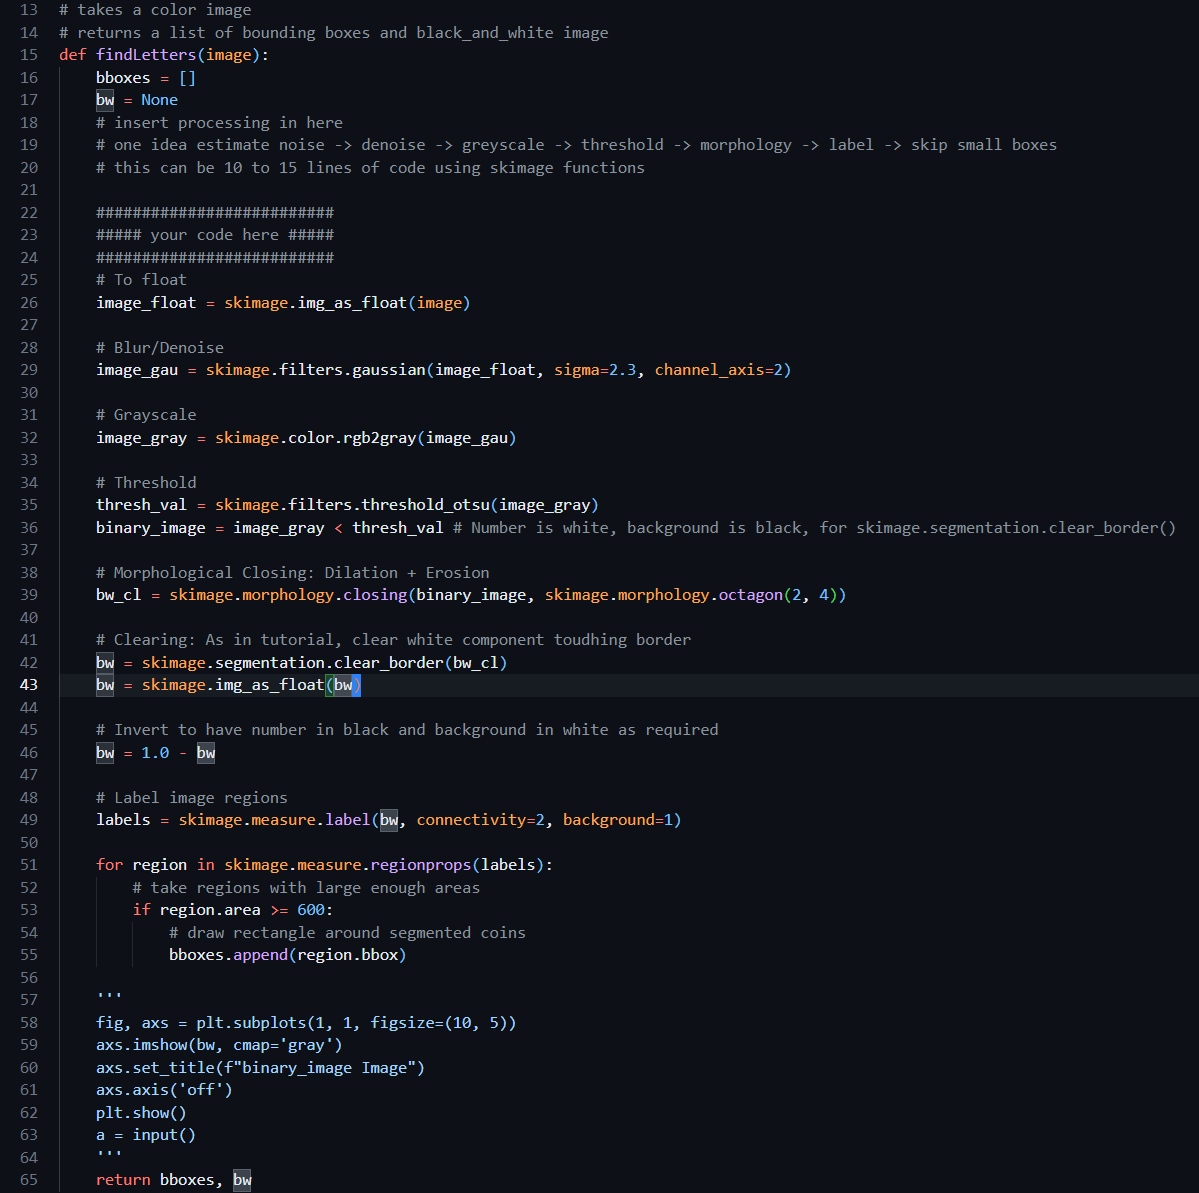
\includegraphics[width=0.7\linewidth]{./Q42_cns.png}  % Adjust the width to 50% of the line width
	\refstepcounter{figure}  % Increment the figure counter
	\newline
	\textbf{Figure \thefigure:} Code Snippet of findLetters() % Manually add a caption/title
	\label{fig:Q42_cns}  % Label for referencing
	\end{minipage}	


	\newpage
	\subsection*{Q4.3 at page 8}
	Ans:\\
	Results are show as the following \autoref{fig:Q43_res1} to \autoref{fig:Q43_res4}.

	\begin{minipage}{0.48\linewidth}
		\centering
		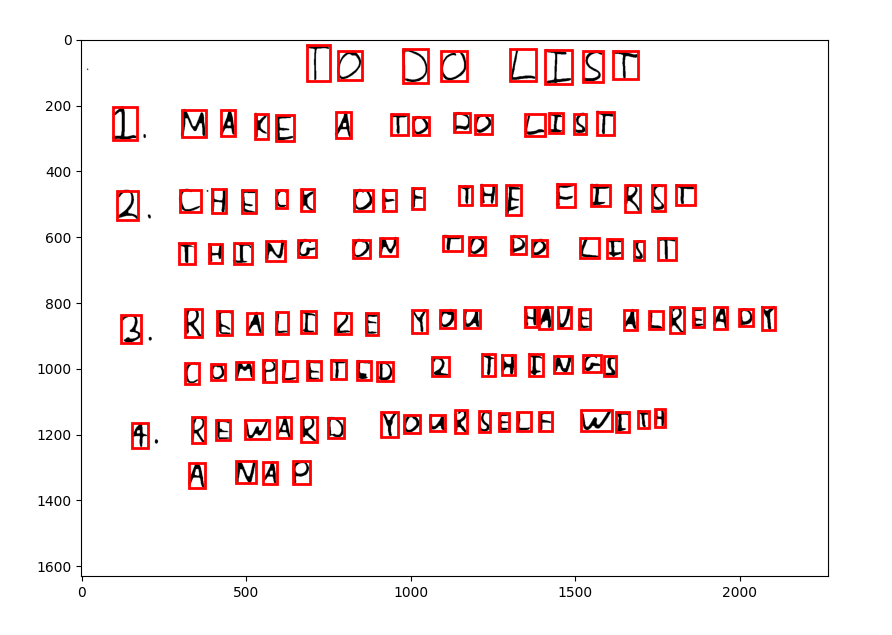
\includegraphics[width=\linewidth]{./Q43_res1.png}
		\refstepcounter{figure}  % Increment the figure counter
		\textbf{Figure \ref{fig:Q43_res1}:} Result of Located Boxes in 01\_list.jpg % Manually add a caption/title
		\label{fig:Q43_res1}         % Label for referencing	
	\end{minipage}
	\hfill
	\begin{minipage}{0.48\linewidth}
		\centering
		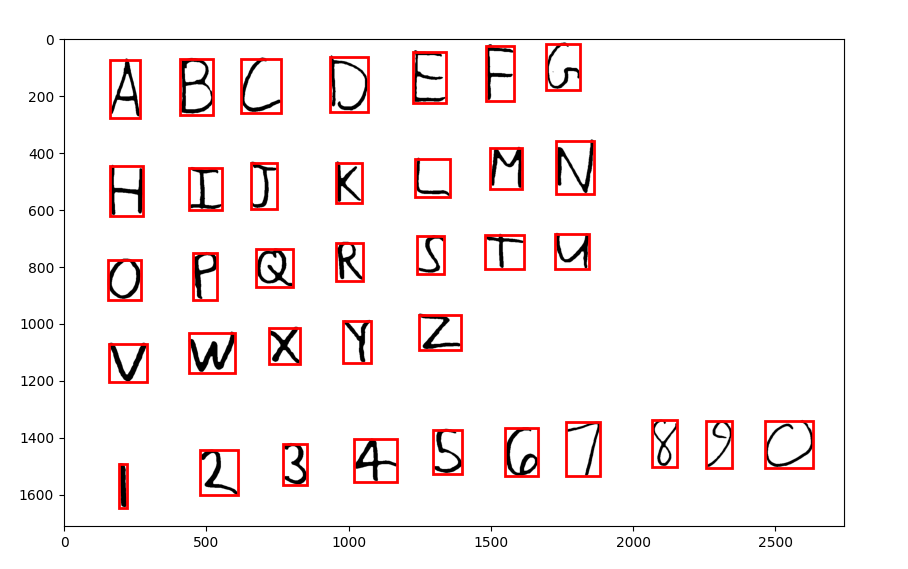
\includegraphics[width=1.1\linewidth]{./Q43_res2.png}
		\refstepcounter{figure}  % Increment the figure counter
		\textbf{Figure \ref{fig:Q43_res2}:} Result of Located Boxes in 02\_letters.jpg  % Manually add a caption/title
		\label{fig:Q43_res2}         % Label for referencing
	\end{minipage}	
	\newline	
	\newline
	
	\begin{minipage}{0.48\linewidth}
		\centering
		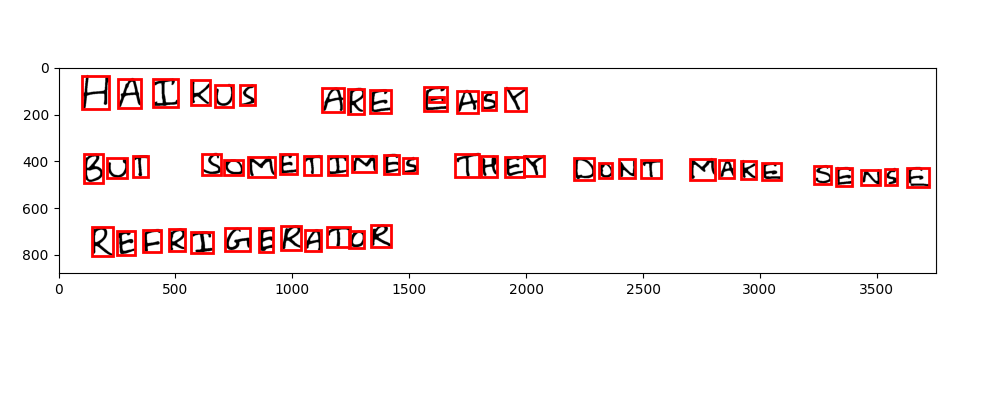
\includegraphics[width=\linewidth]{./Q43_res3.png}
		\refstepcounter{figure}  % Increment the figure counter
		\textbf{Figure \ref{fig:Q43_res3}:} Result of Located Boxes in 03\_haiku.jpg % Manually add a caption/title
		\label{fig:Q43_res3}         % Label for referencing	
	\end{minipage}
	\hfill
	\begin{minipage}{0.48\linewidth}
		\centering
		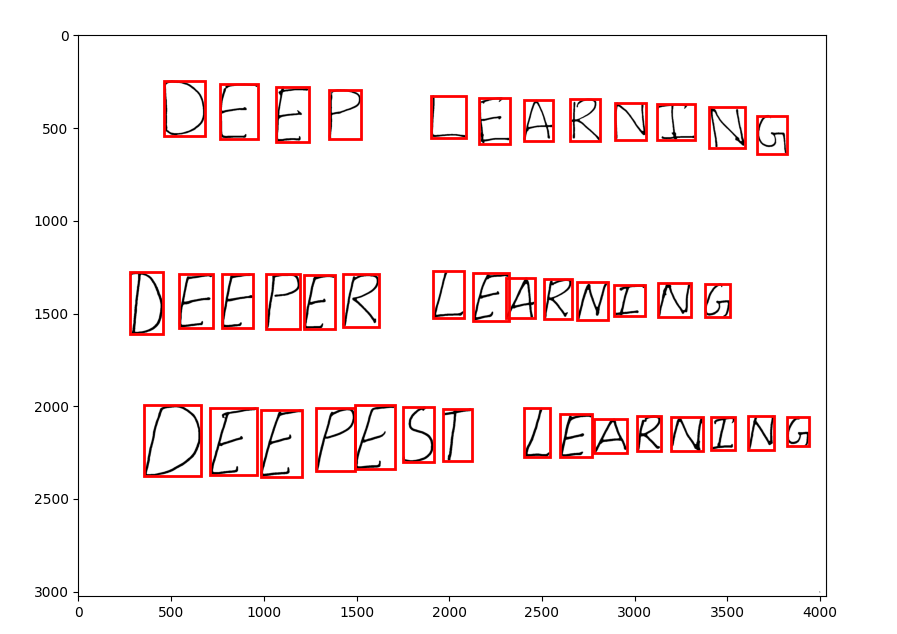
\includegraphics[width=\linewidth]{./Q43_res4.png}
		\refstepcounter{figure}  % Increment the figure counter
		\textbf{Figure \ref{fig:Q43_res4}:} Result of Located Boxes in 04\_deep.jpg  % Manually add a caption/title
		\label{fig:Q43_res4}         % Label for referencing
	\end{minipage}	
	\newline
	
	\newpage
	\subsection*{Q4.4 at page 8}
	Ans:\\
	Results are shown as the following \autoref{fig:Q44_res1} - \autoref{fig:Q44_res4_gt}. The correction rate of 01\_list.jpg is 80.8696\%, the correction rate of 02\_letters.jpg is 83.333\%, the correction rate of 03\_haiku.jpg is 88.889\%, and the 04\_deep.jpg is 85.366\%.
	
\captionsetup{font=scriptsize} 		
\begin{figure}[H]
	\centering
	\begin{minipage}{0.33\linewidth}
		\centering
		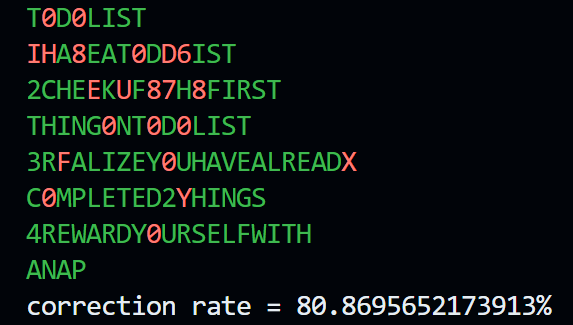
\includegraphics[width=\linewidth]{./Q44_res1.png}
		\caption{Output result of the model.}
		\label{fig:Q44_res1}
	\end{minipage}%
	\hfill
	\begin{minipage}{0.33\linewidth}
		\centering
		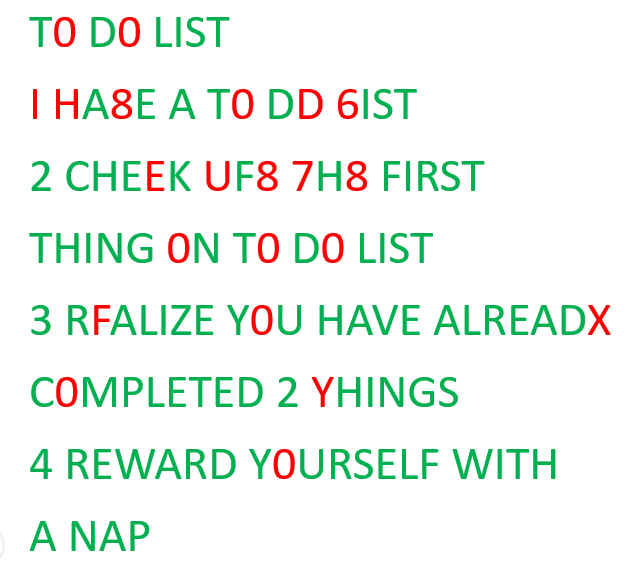
\includegraphics[width=\linewidth, height=0.56\columnwidth]{./Q44_add_space1.png}
		\caption{Add space back to the result.}
		\label{fig:Q44_add_space1}
	\end{minipage}%
	\hfill
	\begin{minipage}{0.33\linewidth}
		\centering
		\includegraphics[width=\linewidth]{./images/01_list.jpg}
		\caption{Ground Truth: 01\_list.jpg}
		\label{fig:Q44_res1_gt}
	\end{minipage}
\end{figure}

\begin{figure}[H]
	\centering
	\begin{minipage}{0.33\linewidth}
		\centering
		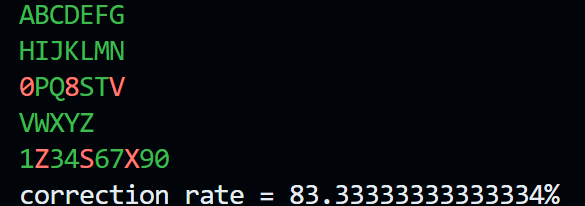
\includegraphics[width=\linewidth]{./Q44_res2.png}
		\caption{Output result of the model.}
		\label{fig:Q44_res2}
	\end{minipage}%
	\hfill
	\begin{minipage}{0.33\linewidth}
		\centering
		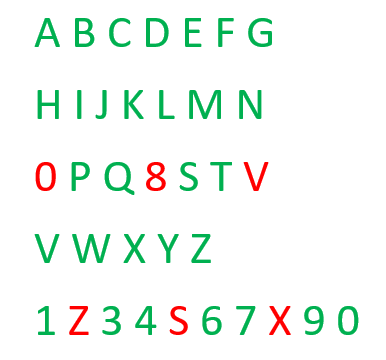
\includegraphics[width=0.6\linewidth, height=0.35\columnwidth]{./Q44_add_space2.png}
		\caption{Add space back to the result.}
		\label{fig:Q44_add_space2}
	\end{minipage}%
	\hfill
	\begin{minipage}{0.33\linewidth}
		\centering
		\includegraphics[width=\linewidth]{./images/02_letters.jpg}
		\caption{Ground Truth: 02\_letters.jpg}
		\label{fig:Q44_res2_gt}
	\end{minipage}
\end{figure}

\begin{figure}[H]
	\centering
	\begin{minipage}{0.33\linewidth}
		\centering
		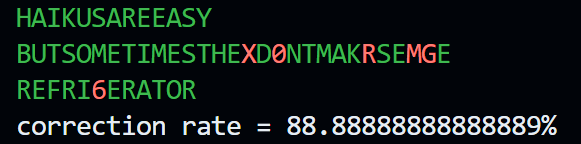
\includegraphics[width=\linewidth]{./Q44_res3.png}
		\caption{Output result of the model.}
		\label{fig:Q44_res3}
	\end{minipage}%
	\hfill
	\begin{minipage}{0.33\linewidth}
		\centering
		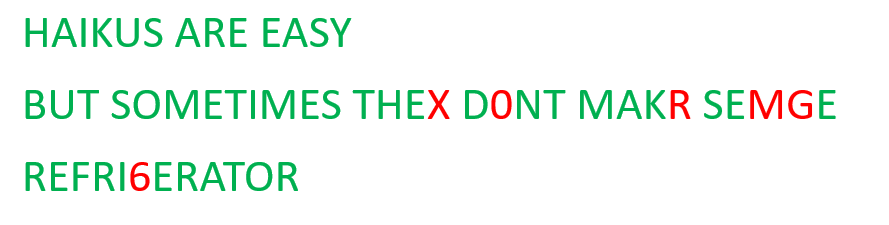
\includegraphics[width=1\linewidth, height=0.25\columnwidth]{./Q44_add_space3.png}
		\caption{Add space back to the result.}
		\label{fig:Q44_add_space3}
	\end{minipage}%
	\hfill
	\begin{minipage}{0.33\linewidth}
		\centering
		\includegraphics[width=\linewidth]{./images/03_haiku.jpg}
		\caption{Ground Truth: 03\_haiku.jpg}
		\label{fig:Q44_res3_gt}
	\end{minipage}
\end{figure}

\begin{figure}[H]
	\centering
	\begin{minipage}{0.33\linewidth}
		\centering
		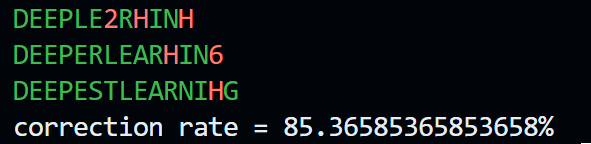
\includegraphics[width=\linewidth]{./Q44_res4.png}
		\caption{Output result of the model.}
		\label{fig:Q44_res4}
	\end{minipage}%
	\hfill
	\begin{minipage}{0.33\linewidth}
		\centering
		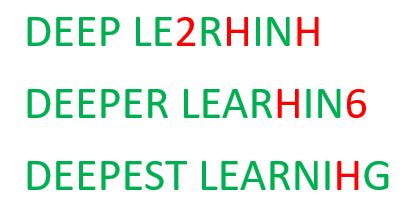
\includegraphics[width=0.8\linewidth, height=0.24\columnwidth]{./Q44_add_space4.png}
		\caption{Add space back to the result.}
		\label{fig:Q44_add_space4}
	\end{minipage}%
	\hfill
	\begin{minipage}{0.33\linewidth}
		\centering
		\includegraphics[width=\linewidth, height=0.6\columnwidth]{./images/04_deep.jpg}
		\caption{Ground Truth: 04\_deep.jpg}
		\label{fig:Q44_res4_gt}
	\end{minipage}
\end{figure}

	\newpage
	
	\subsection*{Q5 at page 8\texttt{}}
	Ans:\\
	\hangindent=1.5em \hspace{1.5em}Two 



	\newpage
	\subsection*{Collaborations}
	Ans:\\
	\hangindent=0.4em \hspace{0.3em} Though I do not have collaborators, I found the following websites helpful on understanding the concepts in this homework.
	\begin{enumerate}
		\item \url{https://www.ri.cmu.edu/pub_files/pub3/baker_simon_2003_3/baker_simon_2003_3.pdf.}
		\item \url{http://16385.courses.cs.cmu.edu/spring2024/lecture/track}
		\item \url{https://stats.stackexchange.com/questions/559575/how-does-addition-of-a-regularization-term-ensures-that-the-matrix-is-nonsingula}
		\item \url{https://docs.opencv.org/4.x/d7/d4d/tutorial_py_thresholding.html}
		\item \url{https://matplotlib.org/stable/api/_as_gen/matplotlib.pyplot.imsave.html}
		\item \url{https://docs.opencv.org/4.x/d4/d61/tutorial_warp_affine.html}		
	\end{enumerate}

\end{document}